\section{Experimental Design and Implementation}
\label{SI_experiment}

The data used in this work come from an experiment that we ran using an experimental platform 
designed to measure how participants form and update causal beliefs in more or less complex 
settings.  The experiment was conducted at Columbia University Social Science laboratory and 
involved 96 subjects.  Upon arrival, subjects were briefed and directed to an individual booth . 
The experiment was performed on a graphical  html/javascript interactive Web interface. All 
actions taken on the interface by subjects were recorded in real-time (resolution : $1s$). 

In the experiment, participants see a data stream: data about multiple binary variables in a 
system, which take on the value High or Low. For example, one variable could be a stock price 
and there may be a number of variables that explain its variation or are explained by its variation 
in turn.  A visual interface allows the subjects to draw a causal model of the system. The platform 
then computes predictions on the basis of the participant's causal model and makes those 
prediction visible to the participant. The participant then makes bets using these predictions. In 
doing so, the participant gets feedback on the accuracy of her beliefs, and can update her beliefs 
by modifying the causal model. The platform thus allows us to observe beliefs and learning in a 
very precise and controlled way.

\subsection{Experimental Treatments}
Data from probabilistic causal systems can be simulated and presented to people so that they may reverse engineer the causal 
structures that generated the patterns that they see. That is, experimental participants see data and build causal models, seeking to 
understand how the data was produced and to make predictions of future observations. \\

To make things concrete yet not obvious , we labeled the variables with names from economics, as these seem to relate to many 
people: "Interest Rate (IR)", "Financial Sector (FS)", "industry (ID)" and "Consumer Spending (CS)". We thus {\bf [simulated]} from the joint distributions of two such systems, one simpler and the other more complex and presented  people with the data and the modeling tools to learn the causal relationships and parameter values in these systems. The simpler system has three variables: "Interest Rate (IR)", "Financial Sector (FS)" and "Industry (ID)", where the "Interest Rate" has a negative effect on the "Industry" and the "Financial Sector" has a positive effect on the "Industry" (our somewhat arbitrary settings).\\

For the simple treatment, the data that the participants observed were generated in the following way: a variable was chosen at 
random from the system's variables to be the current period's "betting variable". The value of this variable was hidden from the 
participants until the end of the period. Participants were incentivised (on hand the well known Becker–DeGroot–Marschak 
method) to predict the value of this variable. Next, the value of the "interest Rate" variable was drawn; "H", with probability $0.5$ 
and "L: with probability $0.5$, followed by the value of the "Financial Sector" variable, with identical probabilities. Lastly, the value of 
the "Industry" variable was drawn according to Judea Pearl's \citep{Pearl88} probabilistic-OR operator, which gives the conditional 
probability:  

\be
P(ID=1|FS=fs, IR=ir) = 1-(1-\pi_{FS})^{fs}(1-\pi_{IR})^{1-ir} ~with ~ \pi_{FS} = \pi_{IR}=0.5
\ee

The more complex system had four variables labeled "Interest Rate (IR)", "Financial Sector (FS)", "Industry (ID)" and "Consumer 
Spending (CS)", where as before the "Interest Rate" has a negative effect on the "Industry" and the "Financial Sector" has a positive 
effect on the "Industry". In addition, in this system the "Industry" and "Interest Rate" also affect "Consumer Spending". "Industry" 
positively and the "Interest Rate" negatively.  Please do not hold us accountable for those choices, we will not defend these 
particular configurations in any way.

The joint distributions of Bayesian Belief Nets can be calculated as the products of the conditional probabilities and the marginal 
probabilities, as follows. For any number of related variables, $X_1, \ldots, X_n$, their joint probability can be calculated as:

\be
P(x_1, \ldots, x_n) = P(x_1 | x_2, \ldots, x_n) \times P(x_2 | x_3, \ldots, x_n) \times \cdots \times P(x_{n-1} |x_n) \times P(x_n).
\ee

For example, remembering that $P(ID=1|FS=fs, IR=ir) = 1-(1-\pi_{FS})^{fs} \times (1-\pi_{IR})^{1-ir}$, where $\pi_{FS}=\pi_{IR}=0.5$, for 
the simple treatment, the joint outcome $FS=H, IR=H, ID=H$ has probability:\\

\ba
P(FS=H, IR=H, ID=H) =\\ 
P(ID=1|FS=H, IR=H) \times P(FS=H) \times P(IR=H) \\
=  \left(1-(1-\pi_{FS})^{1} \times (1-\pi_{IR})^{1-1}\right) \times 0.5^2 =0.125.  
\ea

A frequentist, might simply count membership of the joint buckets and build a model that matches the percentages. Updating her beliefs in this context of a repeating process, a Bayesian could essentially do the same thing by comparing members of the Dirichlet distribution class (for example, depending on priors) by observing, updating and finding the maximum of the posterior distribution of the parameters, known as the pseudo counts. This maximum turns out to approach the $2^k$ dimensional value of the bin counts. Likewise, all conditional distributions could be calculated in this way, but cognitive scientists and computer scientists have recently found this to be computationally more expensive than necessary \citep{Griffith08, Koller03}.  They suggest that instead of calculating $2^k$ parameters for the joint distribution of $k$ binary variables, people and computers should build structural models, where they can update their beliefs for a much reduced number of parameters and obtain the same results. For the model that we used as the simple treatment process, for example, if one has the right structure and the correct idea that $P(ID=1|FS=0, IR=1)=0$, there are four parameters to form beliefs about: $\pi_{FS}, \pi_{IR}, P(FS), P(IR)$. But perhaps, one doesn't see causation in that way and then there are $5$ parameters.  The full joint distribution has eight parameters.  There are thus less parameters to estimate if a causal theory is postulated. The benefit of thinking structurally will increase as the number of variables gets large because most often, the number of causal relationships (structural parameters) increases linearly in the number of variables, $k$, whereas the parameters of the joint distribution increases exactly by $2^k$.  At most, each variable that is added, affects every variable that is already there and then the number of causal arrows grows with $k$ as $k(1-k)$. In light of this, it seems evident that people should have a harder time guessing the correct structure and estimating the correct structural parameters when the system is complex than when it is simple. This, we hypothesized, should lead their models to be more diverse and less accurate in the complex case. 

%\subsection{Causal Reasoning about a set of Binary Variables}

%Here, we describe and informally define the kinds of systems that experimental participants reasoned about as they participated in our experiment on causal reasoning. 

%\subsubsection{The noisy-or operator \citep{Pearl88}}

%For systems with only binary variables we might think of causation in the following way as suggested by Judea Pearl in 1988.  If causation only involves 2 variables, say $A$ and $B$, where $A$ has a positive causal effect on $B$, then things are simple:

%$P(B = 1 | A = 1) = p$, where $p \in [0, 1]$ and 0 otherwise.  That is, if the cause is present, $B=1$ follows with probability $p$, else it never happens, as there is only one possible cause for $B$ to assume the value $1$ and that is for $A$ to assume the value $1$. Note that in reverse this will mean $P(A=1|B=1)=1$. $B$ can only assume the value $1$ when $A$ is $1$ and thus observing that $B$ is $1$ tells us that $A$ must be $1$ as well. The cookies are gone and there was only one person here who could have eaten them! 

%Other definitions have it that a causal effect of A on B is positive if $P(B = 1 | A = 1) > P(B = 1 | A = 0)$ and $P(B = 0 | A = 1) < P(B = 0 | A = 0)$, but that suggests that there are some ommitted causes of the event $B=1$. 

%Keeping with Judea Pearl's 1986 reasoning, we ask how best to think about causation when there are two binary causes, $B$ and $C$ and one binary outcome. We then generalize this idea. 

%The naive way to pose that would be as:

%$P(A=1|B=b, C=c) = \pi_B \times b + \pi_C \times c$, 

%where $b, c \in \{1, 0\}$ are the values taken on by the variables $B$ and $C$ and $\pi_B$, $\pi_C \in [0,1]$ are the causal effects of $B$ on $A$ and $C$ on $A$ respectively. But the problem with this formulation -- as Pearl pointed out -- is that, since $P(A=1|B=b, C=c)$ is a probability, as such it must take a value between $0$ and $1$.

%The constraint $0< \pi_B \times b + \pi_C \times c <1$ induces a dependence between the causal effects $\pi_B$ and $\pi_C$ that we had not explicitly intended in our theory, which posed that $B$ and $C$ each independently cause $A$. Our implicit theory takes the following explicit form \citep{Pearl88}:

%$P(A=1|B=b, C=c) = 1-(1-\pi_B)^b(1-\pi_C)^c$.

%Pearl called it the noisy-OR operator because, supposing $\pi_B=\pi_C=1$, $A$ will be $1$ exactly whenever $B=1$, $C=1$, or both.  When $\pi_B, \pi_C \in (0, 1)$, the OR operator is noisy. The noisy-OR operator accommodates negative causation and any finite number of causes: 

%$P(A=1|B=b, C=c, D=d) = 1-(1-\pi_B)^b(1-\pi_C)^{1-c}(1-\pi_D)^d$,

%where the exponant, $1-c$ in the term $(1-\pi_C)^{1-c}$ means that the variable $C$ exerts a negative causal influence on the variable $A$.

%For a set of binary variables, then, this simple system defines a causal grammar that allows us to construct almost arbitrary causal structures relating the members of the set.  The only constraint is that one may not propose a model with causal cycles. Such models are logically incoherent, unless we allow for dynamics which we don't in this experiment. Here we're going to restrict ourselves to cases where there are no dynamics, there is just a process that repeats in time, like the proverbial coin flip, but with more or less intricate (complex) internal structures.



%As a side note, it would be interesting so see how labeling could affect learning and diversity.  It can for example be postulated and I find it likely that it is hard for certain people to learn certain relationships because of the meaning that is attached to labels.  Note that I did not include "Taxes" as a variable lable, as this label is a likely candidate to induce hard learning.    






\section{Experiment}
\label{si:experiment}

\section{Jump Sizes $\Delta r$}

Euclidean distance : 

\begin{equation}
\Delta r = d(p, q) = \sqrt{(p_1- q_1)^2 + (p_2 - q_2)^2+\cdots+(p_i - q_i)^2+\cdots+(p_n - q_n)^2}.
\end{equation}

with $n=8$ (3-nodes BayesNet) or $n=16$ (4-npdes BayesNet) and $p$,$q$, 2 consecutive position vectors

\begin{figure}[h!]
\begin{center}
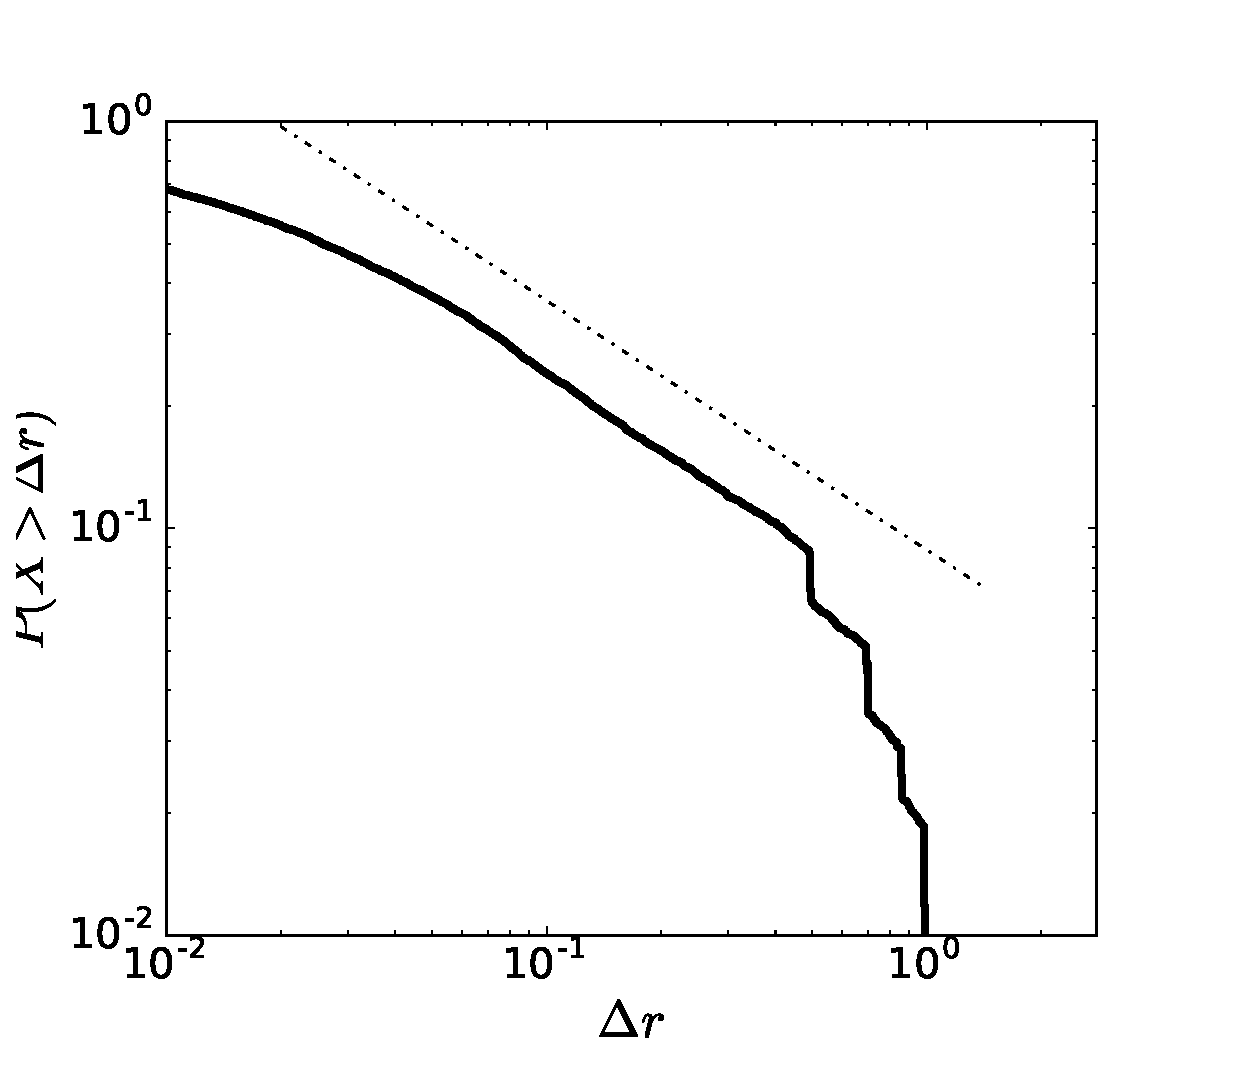
\includegraphics[width=10cm]{figures/CCDF_Displacement_simple.eps}
\caption{(3-node BayesNet) : exponent $\alpha = 0.61(3)$ with upper cutoff  $x_{max} \approx 1.4$ (theoretical limit is $x_{max} = 2\sqrt{2}$).}
\label{fig:jump_sizes}
\end{center}
\end{figure}


\section{Waiting Times $\Delta t$}



\begin{figure}[h!]
\begin{center}
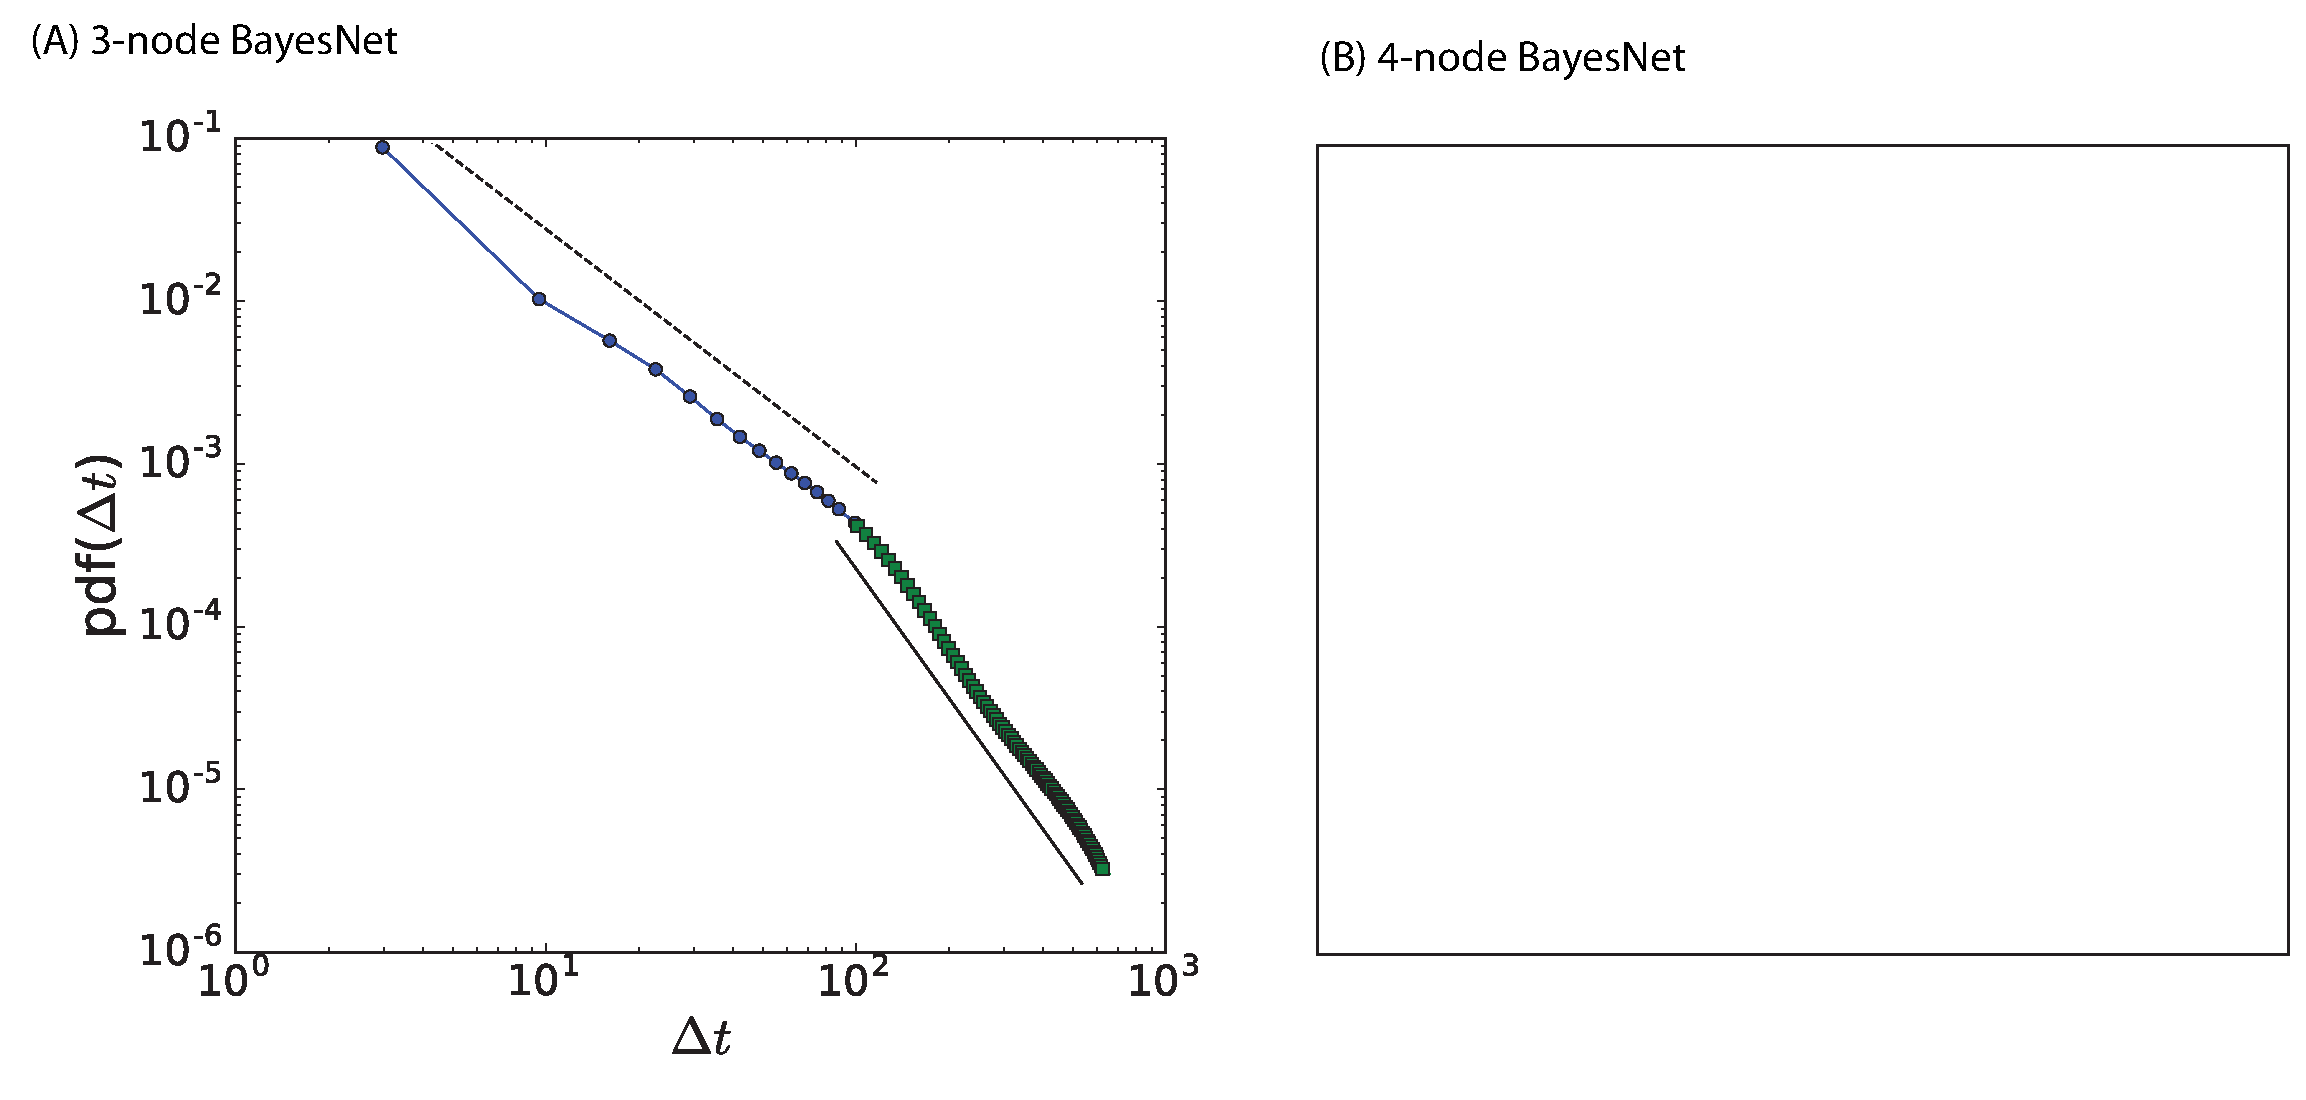
\includegraphics[width=15cm]{figures/dt_kernel_SI.eps}
\caption{Distribution of Waiting Times (fitted by kernel density estimators \cite{}) exhibits a change of regime typical of changes of regimes in waiting times \cite{maillart2011,saichevTheory}: $\beta_{\Delta t  \leqslant 100} \approx 0.46(3)$ (slope $\sim t^{-(1+ \beta_{\Delta t  \leqslant 100})}$ represented by dashed line) and $\beta_{\Delta t > 100} \approx 1.65(1)$ (slope $\sim t^{-(1+ \beta_{\Delta t  > 100})}$ represented by continuous line).}
\label{fig:waiting_times}
\end{center}
\end{figure}


\section{Correlation $\Delta r$ and $\Delta t$}
\label{si:corr_dr_dt}


\begin{figure}[h!]
\begin{center}
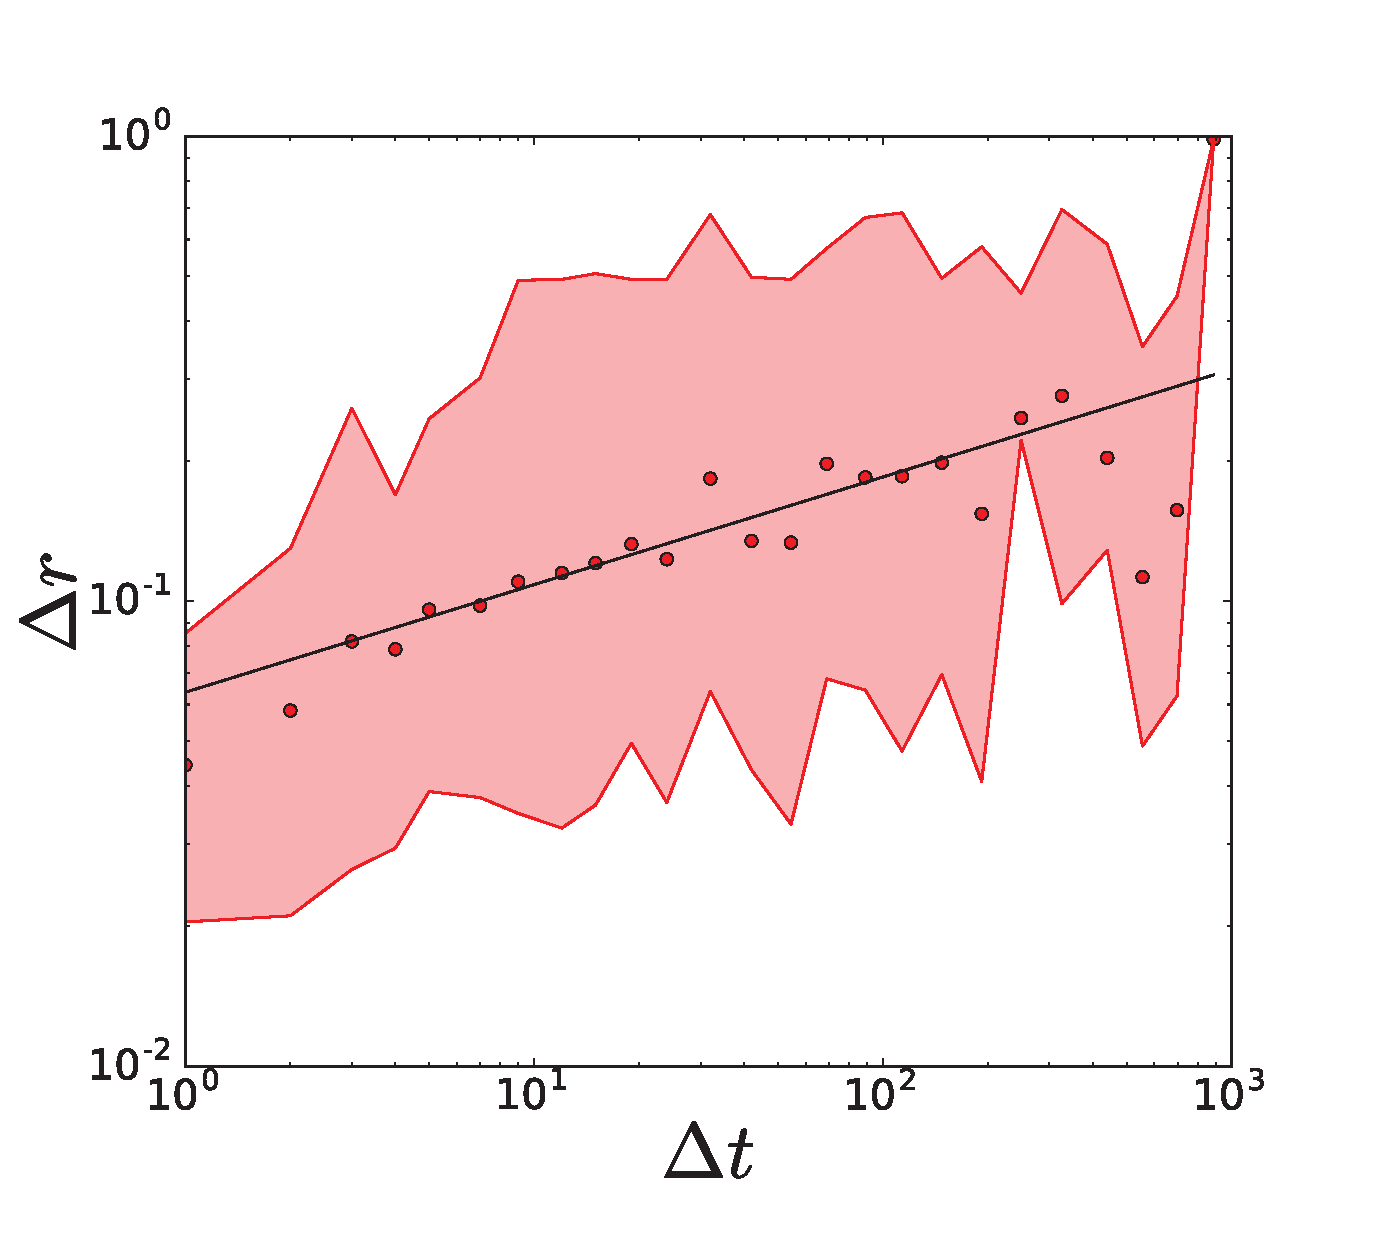
\includegraphics[width=10cm]{figures/cor_Delta_t_Delta_r_simple.eps}
\caption{3-node BayesNet : Correlation (Spearman rank correlation) between $corr(\Delta r,\Delta t) \approx 0.32$, and the main direction of dependence can be approximated by a scaling function $\Delta r \sim {(\Delta t)}^{0.23(2)}$ (least square fit of values in double logarithmique scale, $p < 0.001$ and $R= 0.21$}
\label{fig:corr_dr_dt}
\end{center}
\end{figure}




